\documentclass[12pt]{article}
\usepackage[nolist]{acronym}
\usepackage{commath}
\usepackage{graphicx}
\usepackage{verbatim}
\usepackage{listings}
\usepackage{enumitem}
\title{\vspace{-2cm}Software Specification\vspace{-1cm}} 
\date{}
\begin{document}
\begin{acronym}
	\acro{FPGA}{Field Programmable Gate Array}
	\acro{FIFO}{First In, First Out}
	\acro{CNN}{Convolutional Neural Network}
\end{acronym}
\maketitle
\section{Introduction}
The communication between the host system and the Xillybus embedded Linux system (Xillinux) running on the Zedboard is over Ethernet. Different types of data need to be transmitted:
\begin{itemize}
	\item The updated weights for the neural network from the host to the Zedboard, as long as the training is running on the host, as well as the output errors
	\item The 28x28 input images showing digits between 0 and 9
\end{itemize}
Further, this information needs to be processed and then sent from the ARM processor to the \ac{FPGA} over the Xillybus \ac{FIFO} data streams. 

A remote connection to the Xillinux system can be established over UART.
\section{Top-Level Description}
\begin{figure}[h] 
	\centering
	{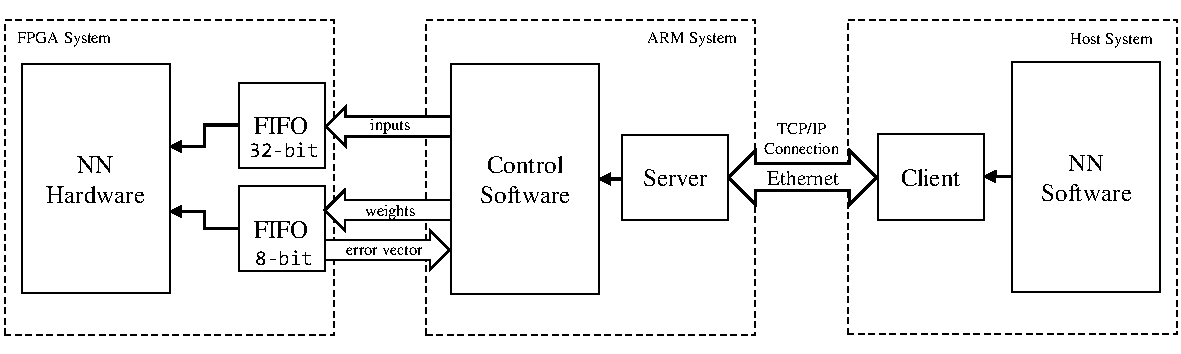
\includegraphics[scale=0.7]{img/toplevel.pdf}} 
	\caption{Top level description}
\end{figure} 
\section{File Tree}
\begin{figure}[h] 
	\centering
	{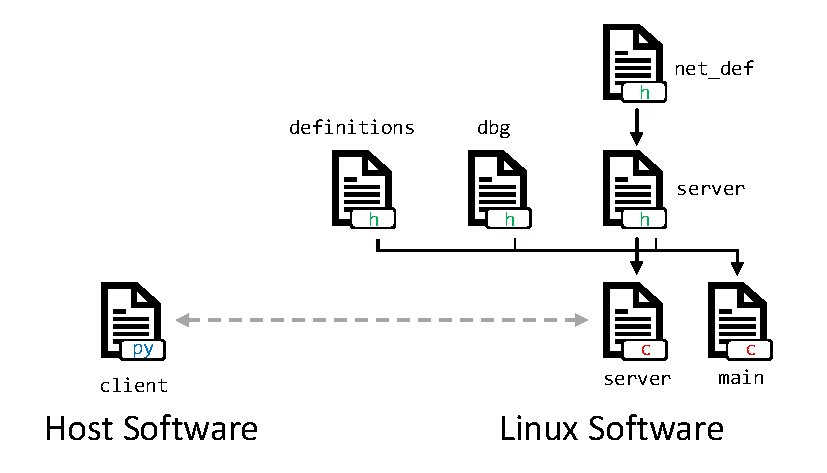
\includegraphics[scale=0.75]{img/software.pdf}} 
	\caption{File tree for the software}
\end{figure} 
\begin{itemize}
	\item \verb|net_def.h| Contains definitions for networking, e.g. ports used.
	\item \verb|dbg.h| Contains debugging macros for logging and error handling.
	\item \verb|definitions.h| Contains information about the neural network, e.g. the number and type of \ac{CNN} stages, layers in the fully connected network, input size and so on.
	\item \verb|server.{c,h}| Handles the connection with the host software.
	\item \verb|main.c| Contains the \verb|main()| function with the main program loop that transmits and manages data to the hardware and from the host system.
	\item \verb|client.py| Handles the connection with the client software.
\end{itemize}
\section{Software Model}
The software running on the host system is written in Python and the embedded software is written in C. The server software should run automatically on start-up.
\subsection{Host}
The host software written in Python essentially just reads the input images and sends them to the board. As long as training is happening on the host, it also receives error data, from which updated weights can be calculated which are then sent back to the system. Otherwise, it receives the final decision about the digit on the inpuit image.
\subsection{Networking}
The embedded Linux distribution running on the board should automatically receive an IP address when connected to a network. When in doubt the address can be found out with the \verb|ifconfig| command. The software has a client-server model with the embedded system acting as a server and the host as a client. Once running, the server software is listening for new outside connections.

On Windows host systems, \emph{Network Discovery} needs to be enabled and in some cases a Firewall exception for the used ports needs to be set for a connection to be established.
\subsection{FPGA Communication}
The Linux system can communicate with the \ac{FPGA} hardware over data streams which are in fact abstractions of \ac{FIFO} buffers. For this, three \ac{FIFO}s are in use:
\begin{itemize}
	\item \verb|/dev/xillybus_write_32|\newline
	This stream is used to write the input images and updated coefficients to the \ac{FPGA} logic.
	\item \verb|/dev/xillybus_write_8|\newline
	This stream is used as a control \ac{FIFO} to tell the hardware to either read an image or the new coefficients next.
	\item \verb|/dev/xillybus_read_8|\newline
	This stream is used to read the error vector from the \ac{FPGA} logic when in training mode OR the decision on the decimal number when in deployment.
\end{itemize}
\section{Hardware Requirements}
The hardware should fulfill the following requirements:
\begin{itemize}
	\item Control the interface of the three \ac{FIFO} buffers.
	\item Read the input images from 32-bit write \ac{FIFO}, 28x28 byte at a time (full image) which is equal to 196x32 bits.
	\item Read the updated coefficients (if training is on host) and set them in the logic. The hardware needs to know how many bytes are to be read.
	\item Write the error vector back to the 8-bit \ac{FIFO} (if training is on host), which should equal 10 bytes.
	\item If updated coefficients are available in the \ac{FIFO} buffer, they should immediately be applied to the whole network as soon as the image that is currently processed is done.
\end{itemize}
The \ac{FIFO}s have the following signals: \verb|wr_en| or \verb|rd_en|, 32 or 8-bit \verb|data|, \verb|full| and \verb|empty|. It is a plain \ac{FIFO} and not a first-word fall-trough \ac{FIFO}, which means that on a clock cycle where \verb|empty| is 0, \verb|rd_en| needs to first be asserted for one clock cycle before the data is read in the following clock cycle.
\section{Software Requirements}
The host software should fulfill the following requirements:
\begin{itemize}
	\item Read the error vector and compute new coefficients which are then sent back OR receive the decision from the neural network and generate statistics about the accuracy.
	\item Do not send so many input images as to overflow the buffers of the control software running on the ARM. The number of error vectors or results received back from the board should serve as a method to find out how many 
\end{itemize}
\end{document}